\vspace{-0.1in}
\section{Causal Framework for Reward Modeling}
\label{sec:preliminaries}

\vspace{-0.05in}



\begin{figure}[!t]               % one float, two columns inside
  \centering
  \begin{minipage}[t]{0.58\textwidth}
    \vspace{0.0in}
    \centering
    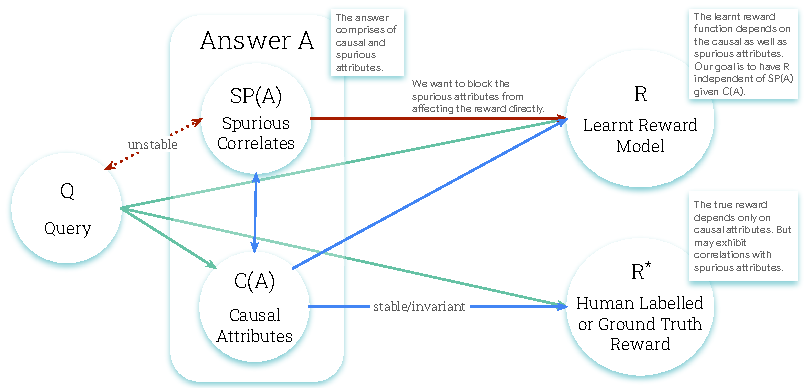
\includegraphics[width=\linewidth]{images/CausalGraphA.pdf}

  \end{minipage}\hfill
  \begin{minipage}[t]{0.4\textwidth}
        \centering
        \vspace{-0.25in}
        \resizebox{\linewidth}{!}{
        \begin{tabular}{c|p{0.75\linewidth}}
\toprule
\textbf{Path/ Relationship} & \textbf{Interpretation Summary} \\
\midrule
$(\mathrm{Q}, \mathrm{C}(\mathrm{A})) \to \mathrm{R}^*$ & Ground-truth reward $\mathrm{R}^*$ determined by query $\mathrm{Q}$ and causal attributes $\mathrm{C(A)}$; stable relationship. \\
$\mathrm{Q} \leftrightarrow \mathrm{SP(A)}$  & Query $\mathrm{Q}$ and unknown spurious attributes $\mathrm{SP(A)}$ are correlated/confounded by unstable exogenous factors. \\
$\mathrm{Q} \to \mathrm{C(A)}$ & Query $\mathrm{Q}$ determines relevant causal attributes $\mathrm{C(A)}$. \\
$\mathrm{SP(A)} \leftrightarrow \mathrm{C(A)}$ & Bidirectional (potentially complex) relationship between spurious $\mathrm{SP(A)}$ and causal $\mathrm{C(A)}$ attributes. \\
\bottomrule
\end{tabular}
        }
        \label{tab:causal_arrows}
  \end{minipage}\hfill

\caption{Conceptual Causal Graph for Reward Modeling. $\mathrm{Q}$ is the query. Answer (A) has causal attributes $\mathrm{C}(\mathrm{A})$ and spurious attributes $\mathrm{SP}(\mathrm{A})$. $\text{dim}(C(A)) \ll \text{dim}(SP(A))\ \forall A$. $\mathrm{SP(A)}$ is unknown. Ground-truth reward $\mathrm{R}^*$ depends only on $\mathrm{C(A)}$ and $\mathrm{Q}$ ($\mathrm{R^*} \perp \mathrm{SP(A)} | \mathrm{C(A)}$, Q). Augmentations heighten $\hat{\mathrm{R}}_\theta$'s sensitivity to $\mathrm{C(A)}$ (approximated by oracle LLM).}
\label{fig:causal_graph}
\vspace{-0.15in}
\end{figure}


\vspace{-0.05in}
We aim to develop a reward model that accurately assesses the quality of an answer $\mathrm{A}$ provided in response to a query $\mathrm{Q}$. Our approach is grounded in a causal framework designed to distinguish genuine quality drivers from spurious correlates often present in preference data. This involves understanding the answer generation process and strategically augmenting training data with approximated counterfactual examples.

\vspace{-0.1in}
\subsection{Reward Model and Pairwise Preferences}
We train a reward model (RM), denoted $\hat{\mathrm{R}}_\theta(\mathrm{Q}, \mathrm{A})$, to assign a scalar quality score to an answer $\mathrm{A}$ for a query $\mathrm{Q}$. This RM is typically optimized on a dataset  preferences pairs $\mathcal{D}_{\mathrm{pref}} = \{(\mathrm{Q}^{(i)}, \mathrm{y}_w^{(i)}, \mathrm{y}_l^{(i)})\}_{i=1}^N$. Given a pair of answers $(\mathrm{A}_1, \mathrm{A}_2)$, the probability of $\mathrm{A}_1$ being preferred over $\mathrm{A}_2$ is commonly modeled using the Bradley-Terry framework \citep{bradley1952rank}:
\begin{equation}
\mathrm{P}(\mathrm{A}_1 \succ \mathrm{A}_2 | \mathrm{Q}; \theta) = \sigmoid(\hat{s}_\theta(\mathrm{Q}, \mathrm{A}_1) - \hat{s}_\theta(\mathrm{Q}, \mathrm{A}_2)) = \frac{\exp(\hat{s}_\theta(\mathrm{Q}, \mathrm{A}_1))}{\exp(\hat{s}_\theta(\mathrm{Q}, \mathrm{A}_1)) + \exp(\hat{s}_\theta(\mathrm{Q}, \mathrm{A}_2))}
\label{eq:bt_prob_roman}
\end{equation}
where $\hat{s}_\theta(\mathrm{Q}, \mathrm{A})$ represents the underlying scalar score (or logit) assigned by the model to answer $\mathrm{A}$ for query $\mathrm{Q}$. \footnote{The score $\hat{s}_\theta(\mathrm{Q}, \mathrm{A})$ can be the direct output of a reward head or, in some pairwise preference models, $\hat{s}_\theta(\mathrm{Q}, \mathrm{A}_1) - \hat{s}_\theta(\mathrm{Q}, \mathrm{A}_2)$ might be directly modeled as the logit of preferring $\mathrm{A}_1$ over $\mathrm{A}_2$.} The parameters $\theta$ are learned by minimizing the negative log-likelihood of  preferences.


\begin{table}[!t]
\centering

\vspace{-0.1in}
\vspace{1em}
\newcolumntype{L}{>{\raggedright\arraybackslash}p{4.0cm}}
\newcolumntype{P}{>{\raggedright\arraybackslash}p{6.0cm}}
\newcolumntype{C}{>{\centering\arraybackslash}p{1.3cm}} 
\newcolumntype{R}{>{\raggedleft\arraybackslash}p{2.5cm}}  

\begin{tabular}{@{}l L P C R@{}}
\toprule
\textbf{Category} & \textbf{Strategy} & \textbf{Generation Pair Example} & \textbf{Assigned Label} & \textbf{Training Objective ($\mathrm{P}_\theta$)} \\
\midrule
\multicolumn{5}{l}{\textit{Causal Augmentation} ($\mathcal{D}_{\mathrm{causal}}$) - Enhancing Sensitivity to $\mathrm{C}$} \\
\midrule
Causal & Attribute Upgradation/Degradation & $(\tilde{\mathrm{A}}_{(C_j \leftarrow \text{upgraded})}, \mathrm{A})$ \textbf{or} $(\mathrm{A}, \tilde{\mathrm{A}}_{(C_j \leftarrow \text{degraded})})$ \newline  & $\succ$ & $\to 1$ \\

\midrule
\multicolumn{5}{l}{\textit{Neutral Augmentation} ($\mathcal{D}_{\mathrm{neutral}}$) - \textit{Enforcing Invariance to} $\mathrm{SP}$} \\
\midrule
Neutral & Pairing with Irrelevant Queries & $(\mathrm{B}_1, \mathrm{B}_2)$ with new $\mathrm{Q}_{\text{irrelevant}}$ \newline \footnotesize{s.t. $\mathrm{C(B_1|Q_{\text{irrelevant}})} \approx \mathrm{C(B_2|Q_{\text{irrelevant}})} \approx \mathbf{0}$} & $ \approx $ (tie) & $\approx 0.5$ \\
\bottomrule
\end{tabular}
\caption{Summary of \carma{}'s synthetic data augmentation strategies using LLM-approximated counterfactuals. $\tilde{\mathrm{A}}_{(C_j \leftarrow \text{target})}$ signifies an LLM-generated counterfactual of $\mathrm{A}$ with its $j$-th causal attribute $C_j$ modified.\vspace{-0.15in}}
\label{tab:augmentation_summary}
\end{table}

\vspace{-0.05in}
\subsection{A Causal Model of Answer Generation}
\label{subsec:causal_graph}

\vspace{-0.05in}
We propose a causal model (Figure \ref{fig:causal_graph}) for answer generation and quality perception. For a query-answer pair $(\mathrm{Q}, \mathrm{A})$, we distinguish two attribute types:

\vspace{-0.1in}
\begin{itemize}[itemsep=0pt,left=0pt]
    \item \textbf{Causal Attributes} $\mathrm{C}(\mathrm{A}) = \{\mathrm{C}_1, \dots, \mathrm{C}_\ell\}$: Fundamental quality dimensions (e.g., factuality, relevance) genuinely determining quality relative to $\mathrm{Q}$.
    \item \textbf{Spurious Attributes} $\mathrm{SP}(\mathrm{A}) = \{\mathrm{SP}_1, \dots, \mathrm{SP}_k\}$: Other features (e.g., length, formatting) correlated with preferences or $\mathrm{Q}$ in $\mathcal{D}_{\mathrm{pref}}$, but not intrinsically determining quality. $\mathrm{SP}(\mathrm{A})$ can be high-dimensional and unknown.
\end{itemize}

\vspace{-0.1in}
The ground-truth reward $\mathrm{R}^*(\mathrm{Q}, \mathrm{A})$ is assumed to be solely a function of causal attributes: $\mathrm{R}^*(\mathrm{Q}, \mathrm{A}) = f^*(\mathrm{Q}, \mathrm{C}(\mathrm{A}))$. This implies conditional independence: $\mathrm{R}^* \perp \mathrm{SP}(\mathrm{A}) | \mathrm{Q}, \mathrm{C}(\mathrm{A})$.

We explicitly assume the following stability property: \textit{If the entire process of answer generation and reward labeling were repeated (e.g., with a different labeler or answer generator), the relationship $(\mathrm{Q}, \mathrm{C}(\mathrm{A})) \to \mathrm{R}^{*}$ determining the reward is stable/invariant.} In contrast, correlations involving $\mathrm{SP}(\mathrm{A})$ (e.g., $\mathrm{SP}(\mathrm{A}) \leftrightarrow \mathrm{C}(\mathrm{A})$ or $\mathrm{SP}(\mathrm{A}) \leftrightarrow \mathrm{Q}$) can arise from various, potentially unstable or unknown exogenous factors, and thus these correlations may vary across such repetitions.

The primary challenge is that standard reward models $\hat{\mathrm{R}}_\theta$ may inadvertently learn high sensitivity to these unstable correlations with $\mathrm{SP}(\mathrm{A})$ (due to its unknown, high-dimensional nature). Our goal is to train $\hat{\mathrm{R}}_\theta$ such that its dependence on $\mathrm{A}$ is primarily mediated through the identified, stable causal attributes $\mathrm{C}(\mathrm{A})$, ensuring robustness to unspecified $\mathrm{SP}(\mathrm{A})$.







\vspace{-0.15in}
\subsection{Approximating Counterfactuals for Attribute Intervention}
\label{subsec:approximating_counterfactuals}
\vspace{-0.1in}

To instill causal sensitivity and spurious invariance in $\hat{\mathrm{R}}_\theta$, \carma{} leverages counterfactual reasoning about how answer quality changes if specific attributes were altered. For an answer $\mathrm{A}$ with attributes $(\mathrm{C}(\mathrm{A}), \mathrm{SP}(\mathrm{A}))$, an ideal counterfactual, $A_{(C_j \leftarrow c'_j)}(u)$, would manifest if only its $j$-th causal attribute $C_j$ were set to $c'_j$, considering its causal effects on other features, while all other exogenous factors $u$ (that produced the factual answer $a$) remained constant. Formally, $P_{U}(A_{(C_j \leftarrow c'_j)}(U) | A(U)=a)$.

\vspace{-0.05in}
As generating such ideal textual counterfactuals is intractable, \carma{} employs Large Language Models (LLMs) to produce \textit{approximations}. These LLM-generated answers, denoted $\tilde{\mathrm{A}}_{(C_j \leftarrow \text{target})}$, are rewrites of an original answer $\mathrm{A}$, prompted to modify $C_j$ (e.g., to a ``degraded'' state, lowering reward) while aiming for minimal changes to other attributes.


% \vspace{-0.05in}
\begin{remark}
For brevity, we denote these LLM approximations as $\tilde{\mathrm{A}}_{(C_j \leftarrow c)}$, dropping the explicit $u$ conditioning, assuming the generation approximates such a sample. While imperfect, these approximations provide the targeted variations crucial for our data augmentation.
\end{remark}


\vspace{-0.15in}
\subsection{Augmented Training Data for Causal Disentanglement}
\label{subsec:data_augmentation}


\vspace{-0.1in}
We augment the original preference dataset $\mathcal{D}_{\mathrm{pref}}$ with synthetically generated examples $\mathcal{D}_{\mathrm{aug}}$ designed to enforce specific causal properties on $\hat{\mathrm{R}}_\theta$. This augmented dataset $\mathcal{D}_{\mathrm{aug}}$ comprises two principal categories: Causal Augmentation Pairs ($\mathcal{D}_{\mathrm{causal}}$) and Neutral Augmentation Pairs ($\mathcal{D}_{\mathrm{neutral}}$), summarized in Table \ref{tab:augmentation_summary}.


\begin{figure}[!t]
  \centering
  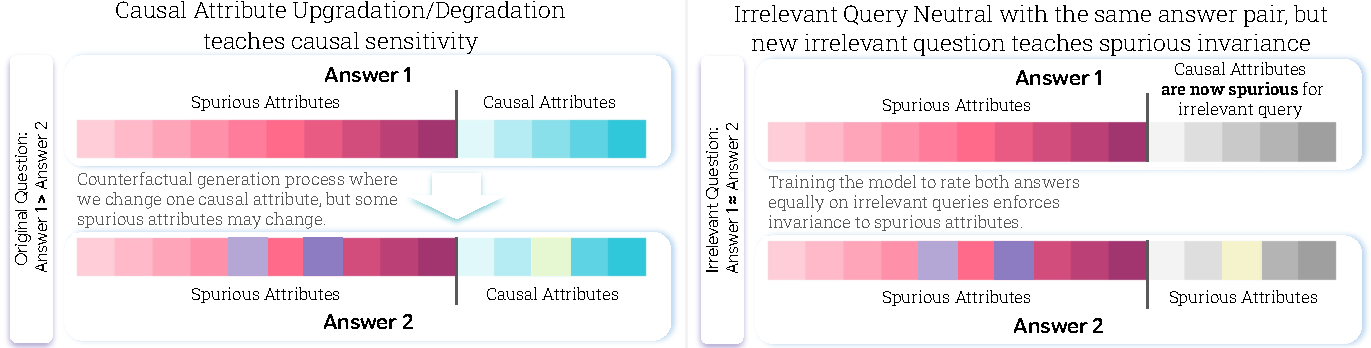
\includegraphics[width=\linewidth]{images/CausalAugmentationProcess_Horizontal.pdf}
  \vspace{-0.2in}

  \caption{Visualizing \carma's core augmentation strategies (detailed in Appendix~\ref{app:detailed_augmentation_diagrams}).
\textbf{(Top) Causal Augmentation:} For a given query, we use an LLM-driven counterfactual generation process to alter a specific causal attribute, yielding Answer 2. Some spurious attributes may co-vary. The RM is trained with a preference (e.g., $A_1 \succ A_2$ if $A_2$ is a degradation), teaching causal sensitivity.
\textbf{(Bottom) Irrelevant Query Neutral:} The same answer pair ($A_1, A_2$) is re-contextualized with a new, irrelevant question. Their original causal attributes become effectively spurious or irrelevant (greyed-out bar). The RM is trained with a tie-label ($A_1 \approx A_2$), teaching invariance to the  attribute differences when no true causal signal for the current query exists. 
This illustrates how IQN provides invariance to those spurious attributes that change with C (like length of response changing with clarity of response).
A similar invariance is imposed using the $(A_1,A_2)$ pairs from the original dataset to provide robustness to general spurious attributes (SP) that do not change with C.\vspace{-0.1in}}
\label{fig:carma_augmentation_visual_overview}
  
\end{figure}



\subsubsection{Causal Augmentation Pairs}

\carma{}'s strategy causal pairs $\mathcal{D}_{\mathrm{causal}}$ focus on isolating the impact of important causal attributes.

\paragraph{Attribute Upgradation and Degradation.}
For an original answer $\mathrm{A}$ (from $\mathcal{D}_{\mathrm{pref}}$) and a specific causal attribute $\mathrm{C}_j$, we generate LLM-approximated counterfactuals.
If $\mathrm{A}$ is of lower quality regarding $\mathrm{C}_j$, we create an upgraded version $\tilde{\mathrm{A}}_{(\mathrm{C}_j \leftarrow \text{upgraded})}$. The pair $(\tilde{\mathrm{A}}_{(\mathrm{C}_j \leftarrow \text{upgraded})}, \mathrm{A})$ is added to $\mathcal{D}_{\mathrm{causal}}$ with label $\tilde{\mathrm{A}}_{(\mathrm{C}_j \leftarrow \text{upgraded})} \succ \mathrm{A}$ post-verification.
Conversely, if $\mathrm{A}$ is of higher quality on $\mathrm{C}_j$, we generate a degraded version $\tilde{\mathrm{A}}_{(\mathrm{C}_j \leftarrow \text{degraded})}$. The pair $(\mathrm{A}, \tilde{\mathrm{A}}_{(\mathrm{C}_j \leftarrow \text{degraded})})$ is added to $\mathcal{D}_{\mathrm{causal}}$ with label $\mathrm{A} \succ \tilde{\mathrm{A}}_{(\mathrm{C}_j \leftarrow \text{degraded})}$.
These pairs collectively teach $\hat{\mathrm{R}}_\theta$ sensitivity to changes along individual causal dimensions.


\subsubsection{Neutral Augmentation Pairs}

Neutral Augmentation Pairs, $\mathcal{D}_{\mathrm{neutral}}$ (with tie-labels) teach invariance to $\mathrm{SP}(\mathrm{A})$ when $\mathrm{C}(\mathrm{A})$ is held constant/ is irrelevant.
\vspace{-0.1in}
\paragraph{Irrelevant Query Neutrals (IQN)} We pair two answers, $\mathrm{B}_1, \mathrm{B}_2$ (from $\mathcal{D}_{\mathrm{pref}} \cup \mathcal{D}_{\mathrm{causal}}$), with a \textit{new, unrelated query} $\mathrm{Q}_{\text{irrelevant}}$. This makes their causal attributes w.r.t. $\mathrm{Q}_{\text{irrelevant}}$ (i.e., $\mathrm{C(B_1|Q_{\text{irrelevant}})}, \mathrm{C(B_2|Q_{\text{irrelevant}})}$) minimal. The pair $(\mathrm{B}_1, \mathrm{B}_2)$ under $\mathrm{Q}_{\text{irrelevant}}$ receives a tie-label, training the RM to disregard spurious differences when causal relevance is absent. Their causal distinction becomes moot, isolating spurious variations under $\mathrm{Q}_{\text{irrelevant}}$. Presenting these as tied responses to the reward model enforces invariance to such spurious attributes.
We provide various other techniques tested for spurious suppression in Section \ref{ssec:neutral_ablations}.


The rationale for \carma{}'s specific choices are discussed in Appendix \ref{sec:causal_model_details} along with different neutral augmentation strategies we tried out. We provide the prompts for generating neutrals in Section \ref{sec:prompt_templates}.